\documentclass[12pt]{article}

\usepackage{geometry,calc}
\usepackage{amsmath,amssymb,hyperref}

\def\quiztitle{Graded Problem 5}
\def\quizsubtitle{Math 4B,\qquad Spring 2017,\qquad Dr. Paul}
\pagestyle{empty}

\geometry{body={6.5in, 9in}, left=1in, top=1in}
\input{../../AxesFunction.tex}

\newcommand{\be}{\begin{enumerate}}
\newcommand{\ee}{\end{enumerate}}

\everymath{\displaystyle}

\begin{document}

%\hfill Student Name: \rule{2in}{.1pt}\\

%\hfill Section Time (e.g. 8am): \rule{2in}{.1pt}\\

\begin{center}
{\Huge \quiztitle}
\vskip.1in
{\large \quizsubtitle}
\end{center}

\begin{enumerate}

 \item Consider the differential equation $y''+y=0$, whose general solution we already know how to find. Answer the following ``boundary value'' problems. Note that our Existence and Uniqueness Theorem does not necessarily apply in this context.
 \begin{enumerate}
  \item What solution(s) satisfy the conditions $y(0)=4$, $y(\pi/6)=3$?
  \item What solution(s) satisfy the conditions $y(0)=3$, $y(\pi)=4$?
  \item What solution(s) satisfy the conditions $y(0)=0$, $y(2\pi)=0$?
 \end{enumerate}
 
 \item  Consider a floating cylindrical buoy with radius $r$ and height $h$ of uniform density $\rho\leq0.5$g/cm$^3$ (the density of water is 1 g/cm$^3$). The buoy is initially suspended at rest with its bottom at the top surface of the water and is released at $t=0$. Thereafter it is acted upon by two forces: a downward gravitational force equal to its weight $mg=\pi r^2hg\rho$, and an upward buoyancy force equal to the weight of the water it displaces $\pi r^2x g$, where $x(t)$ is the depth of the bottom of the buoy beneath the surface at time $t$.  
  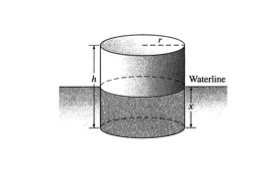
\includegraphics{buoy}
 
 \be
 \item Set up a differential equation describing the motion of the buoy with respect to time. (Ignore water resistance).
 \item Nonzero solutions to the differential equation above should display oscillatory behavior. What is the period of the oscillation (in terms of $r,h,g,\rho$)?
 
 \item Find the solution given the constants $\rho=0.5$ g/cm$^3$, $h=200$ cm, $r=10$ cm, and $g=980$ cm/s$^2$.
 
\ee

 
\end{enumerate}



\end{document}